\documentclass[journal=jctcce,manuscript=article,doi=true]{achemso}
\makeatletter
\acs@doitrue
\makeatother

% Chinese draft support. Remove xeCJK and the font settings for a final
% all-English submission if the submission system does not need them.
\usepackage{xeCJK}
\setCJKmainfont{Songti SC}
\setCJKsansfont{PingFang SC}
\setCJKmonofont{Menlo}

\usepackage{amsmath}
\usepackage{booktabs}
\usepackage{chemformula}
\usepackage{graphicx}
\usepackage{longtable}
\usepackage{multirow}
\usepackage{placeins}
\usepackage{array}
\usepackage{calc}
\usepackage{caption}
\usepackage{listings}
\usepackage{xcolor}

\lstset{
  basicstyle=\ttfamily\small,
  breaklines=true,
  columns=fullflexible,
  keepspaces=true,
  frame=single
}
\providecommand{\passthrough}[1]{#1}
\providecommand{\texorpdfstring}[2]{#1}
\providecommand{\tightlist}{}
\newcommand{\propertycell}[1]{\multirow{6}{=}{\centering #1\par}}

\author{Wenshuo Liang}
\altaffiliation{These authors contributed equally to this work.}
\affiliation[Smartlogic]
{Shanghai Smartlogic Technology Ltd., Shanghai 200040, China}
\author{Yuan Yin}
\altaffiliation{These authors contributed equally to this work.}
\affiliation[SJTU]
{School of Nuclear Science and Engineering, Shanghai Jiao Tong University, Shanghai 200240, China}
\author{Wentao Zhou}
\email{zhwentao@sjtu.edu.cn}
\affiliation[SJTU]
{School of Nuclear Science and Engineering, Shanghai Jiao Tong University, Shanghai 200240, China}
\author{Dezhong Wang}
\affiliation[SJTU]
{School of Nuclear Science and Engineering, Shanghai Jiao Tong University, Shanghai 200240, China}

\title{面向熔盐热物性与输运性质混合阶数外推的物理启发神经模型\\
Physics-Inspired Neural Models for Mixture-Order Extrapolation of Molten Salt Thermophysical and Transport Properties}

\abbreviations{RK,DFT,MD,ML}
\keywords{熔盐, 物理启发机器学习, 热物性与输运性质, 混合阶数外推}

\begin{document}

\begin{abstract}
多组分熔盐的密度、粘度、表面张力和电导率是先进核能、聚光太阳能热储能和高温电化学等应用中的关键物性。然而，三元及更高阶混合物数据稀缺，限制了复杂组成空间中的熔盐体系理性设计与配方优化。本文提出一种物理启发的组分编码神经网络框架，用于从一元和二元熔盐体系学习可迁移的组成---温度---物性关系。模型采用结构化盐组分表示，并在统一的混合阶数外推协议下，比较组成加权--Redlich--Kister 神经混合模型、线性温度约束模型和 Arrhenius 型温度约束模型。本文整合 Janz 熔盐物性汇编和 MSTDB-TP V4.0 数据，采用一元和二元体系训练、三元及以上体系测试的设置进行评估。在三元及以上测试集中，各性质最优模型在相应评价空间中的 Pearson \(r\) 处于 0.93--0.99，表明该框架能够较好保持低阶到高阶混合物的预测趋势相关性。进一步分析显示，不同物性的最优归纳偏置并不相同：密度最受益于低阶 Redlich--Kister 修正，表面张力更适合线性温度约束，粘度中 Arrhenius 型温度约束表现最好，而电导率中 unconstrained model 和 Arrhenius 型模型表现接近。这些结果表明，高阶熔盐物性外推的关键不是引入更复杂或更强的统一物理约束，而是使模型归纳偏置与目标物性的主导机制相匹配。
\end{abstract}

\begin{tocentry}
\centering
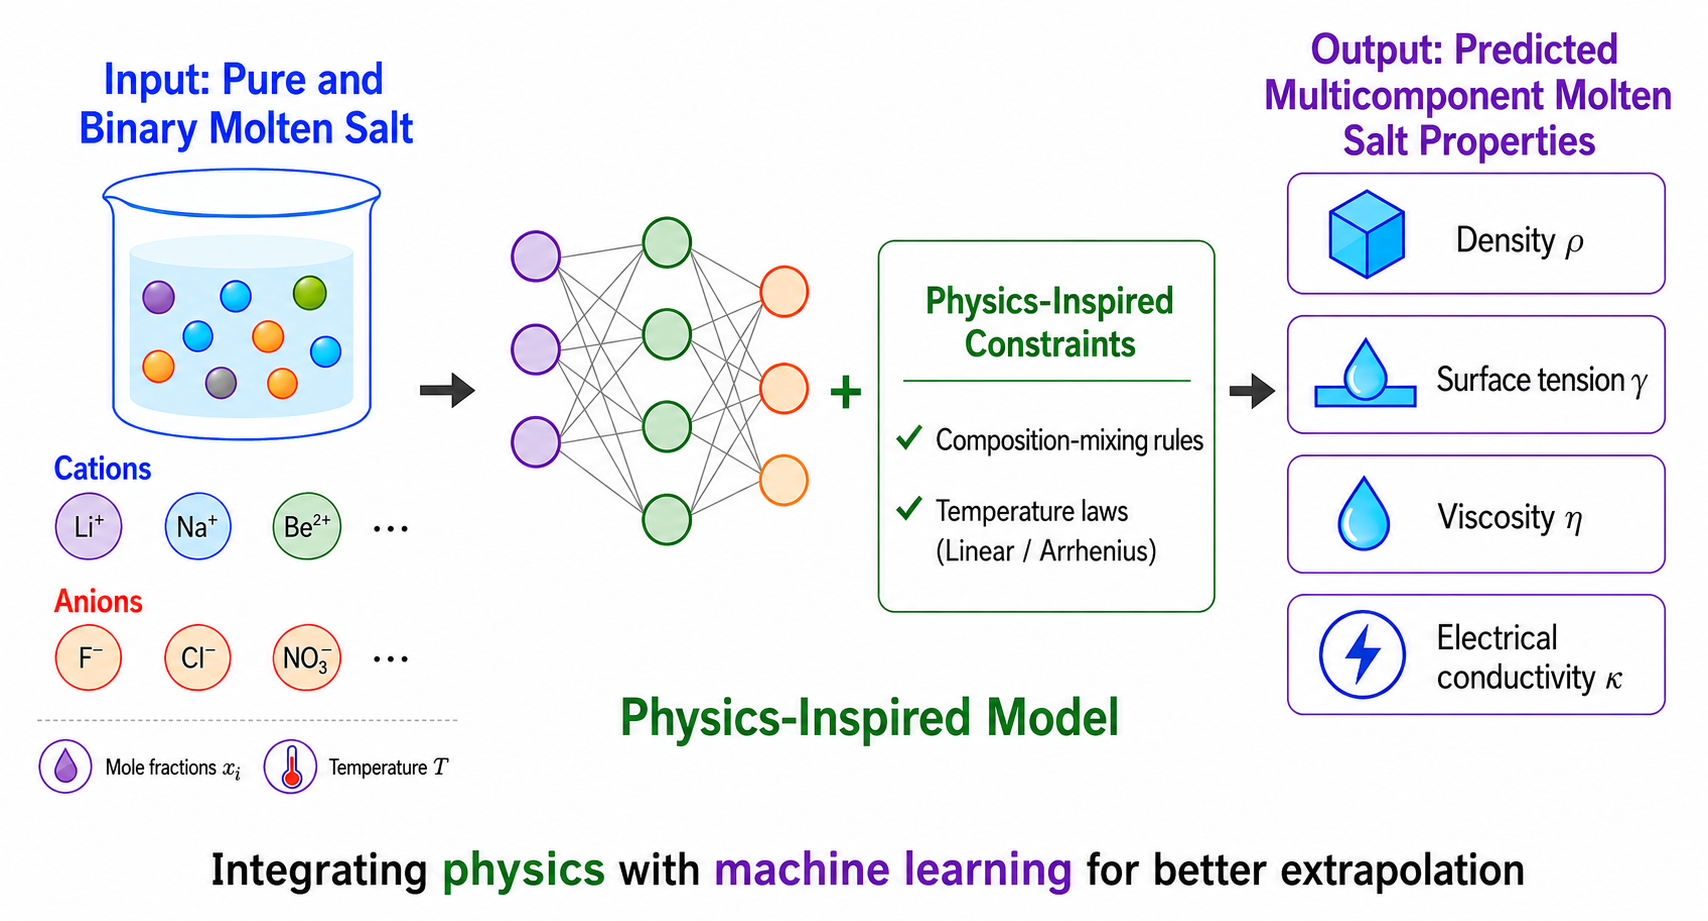
\includegraphics[width=\linewidth]{figures/toc_graphic.png}
\end{tocentry}

\section{引言}\label{ux5f15ux8a00}

熔融无机盐因其高温稳定性、低蒸气压、宽液态温区以及可调的热输运和电化学性质，已成为先进核能系统、聚光太阳能热储能、高温电化学、金属冶炼和材料制备等领域中的重要功能介质 \cite{janz1988molten,roper2022molten,luiz2024review}。在这些应用中，熔盐通常并非以单一纯盐形式使用，而是通过多组分混合来调控熔点、密度、粘度、电导率、腐蚀性和热稳定性。因此，熔盐介质设计本质上是一个多组分组成空间中的物性预测与调控问题，其宏观性质由盐组分、离子类型、化学计量关系、摩尔组成和温度共同决定。在这一背景下，模型不仅需要拟合已有体系的物性数据，还需要学习能够在不同组分组合和温度条件下迁移的组成---温度---物性关系。因此，建立能够基于有限数据预测多组分熔盐性质的模型，是熔盐筛选、工艺设计和系统级传热与流动分析中的基础问题。

为支撑熔盐热物理建模与工程应用，美国 NIST、ORNL 等机构已开展了大量熔盐物性数据汇编、评估和数据库建设工作。Janz 的经典熔盐物性汇编和 NIST Properties of Molten Salts Database (formerly SRD 27) 将密度、粘度、表面张力和电学输运性质作为主要数据类型 \cite{janz1988molten,janz1992nist}。这些性质分别控制体积响应、流动阻力、界面行为和电化学效率，是熔盐热物理与输运建模中的关键参数。然而，熔盐物性数据的获取和泛化建模仍面临显著困难。首先，高温、强腐蚀、吸湿、挥发、杂质敏感性以及容器相容性等因素使实验测量成本高、重复性控制困难，尤其对于含铍、锕系元素或复杂多价金属离子的体系更为明显 \cite{roper2022molten,chesser2025mstdb,magnusson2020review}。其次，已报道数据在组成空间上分布高度不均。NIST SRD 27 覆盖大量无机熔盐物性数据，但多组分体系主要集中于二元混合物，复杂三元及更高阶混合物数据相对有限 \cite{janz1992nist}。ORNL 的 Molten Salt Thermal Properties Database--Thermophysical（MSTDB-TP）持续扩展熔盐热物性数据，其 V4.0 版本进一步整理了密度、粘度、热导率、热容和表面张力等性质 \cite{chesser2025mstdb}，但不同性质、盐族和混合阶数之间的数据覆盖仍不均衡。因此，当前数据缺口并非单纯的样本数量不足，而是低阶体系数据相对丰富、高阶混合物数据系统性稀缺的结构性不均衡。这种不均衡限制了经验关联式和混合规则向复杂组成空间的稳定外推。

在传统建模路线中，熔盐物性预测主要依赖经验关联式、热力学或半经验混合规则以及 CALPHAD 型热化学模型。经验关联式通常针对特定纯盐或混合物建立温度函数，例如密度和表面张力的线性温度关系，以及粘度和电导率中常见的 Arrhenius 型关系。这类关联式形式简洁、便于工程调用，但其参数通常与特定盐种、组成范围和实验温区绑定，因而迁移性较差。CALPHAD 方法和热化学数据库能够提供热力学一致的相平衡、Gibbs 能和反应/混合热力学描述，在熔盐反应堆燃料盐和裂变产物行为分析中具有重要作用 \cite{xiong2022fundamental,besmann2024applications}。然而，此类模型主要面向相平衡和热力学稳定性描述，与本文关注的数据库级工程物性快速预测在建模目标上有所不同。Redlich--Kister（RK）多项式及其扩展形式能够显式描述过量性质和非理想混合效应 \cite{redlich1948algebraic}，并已用于熔融氟盐伪三元体系、氯盐三元体系密度估计以及熔融卤盐粘度估计 \cite{birri2022redlich,birri2024viscosity,agca2022empirical,gallagher2022assessment}。RK 形式的优势在于能够以低阶组成多项式刻画二元非理想性；但其外推瓶颈主要来自交互参数的体系特异性。当二元数据稀缺，或待预测体系包含未充分表征的盐对时，参数可得性和迁移能力受到限制。因此，多元熔盐物性外推的关键问题，是如何在可学习模型中同时表达组分化学信息、摩尔组成、温度依赖和非理想混合效应，从而提升低阶体系到高阶混合物的迁移能力。同时，密度、粘度、表面张力和电导率分别对应体相混合、流动、界面和电学输运等不同物理过程，单一混合规则或单一温度函数是否能够同时适用于这些性质仍缺乏系统评估。

近年来，机器学习方法为熔盐结构---性质建模提供了两类互补路径：一类面向原子尺度势能面学习，另一类面向数据库级的组成---温度---物性直接预测 \cite{porter2022computational,ravichandran2024eutectics}。原子尺度路线的代表性方法是构建机器学习势函数（machine-learning interatomic potentials, MLIPs），如 Behler--Parrinello neural network potential（BPNN）、Deep Potential（DP）\cite{behler2007generalized,zhang2018deep}、NequIP \cite{batzner2022e3} 和 MACE \cite{batatia2022mace}。这类方法通常以 DFT 计算得到的能量、力和应力作为参考数据，训练可近似第一性原理势能面的机器学习势函数，并结合分子动力学模拟进一步预测熔盐热物理与输运性质。近期，Shen 等基于 MACE 构建了面向 11 种阳离子氯盐体系的 MLIP SuperSalt，其在多组分熔盐 MD 模拟中实现了较高精度，在密度预测中相对于 AIMD 和实验数据的平均偏差分别低于 2\% 和约为 5\% \cite{shen2025supersalt}。然而，该路线通常仍依赖大量 DFT 标注数据；例如，SuperSalt 标注了约 \(7.0 \times 10^4\) 个构型以形成训练数据集 \cite{shen2025supersalt}。因此，当前原子级 MLIP 更适合重点体系的高精度模拟和微观机制解析，而难以直接替代面向大规模组成空间筛选的数据库级快速预测模型。

另一类方法直接建立组成---温度---物性之间的监督学习映射，预测成本较低，更适合多组分候选体系的快速筛选和外推评估，也是本文关注的建模层级。Barra 等提出的 chemistry-informed transfer learning 框架利用半经验 RK 关系和 MSTDB-TP 数据训练深度神经网络，用于熔盐混合物密度预测 \cite{barra2025generalizable}。该工作表明，半经验混合关系与化学描述符可以提升熔盐密度建模能力。本文与该方向一致，均强调化学信息和物理启发的归纳偏置在熔盐物性建模中的作用；但本文进一步关注的是，在低阶体系数据可用而高阶混合物数据稀缺的条件下，不同物理启发的归纳偏置能否支持模型稳定迁移到三元及更高阶组成空间。与 Barra 等主要面向密度性质的建模不同，本文同时比较 composition-weighted（CW）RK-style composition-mixing model 和性质特异的 linear/Arrhenius temperature-constrained models。前者用于表达组成加权贡献和成对非理想混合修正，后者用于约束不同物性的温度依赖形式。因此，本文的重点不是证明某一种物理结构能够普遍提升预测精度，而是比较不同归纳偏置在多类熔盐物性低阶到高阶外推中的适用边界。

本文采用混合阶数外推（mixture-order extrapolation）作为核心评估协议，以低阶体系学习、高阶混合物测试的方式，对应高阶熔盐混合物数据系统性稀缺的实际场景。该设置不同于完全 leave-component-out chemical extrapolation：测试体系不要求包含全新的离子或盐组分，而是考察模型能否将低阶体系中学习到的组分贡献、二元相互作用和温度依赖关系组合迁移到更高阶组成空间。

基于上述问题定义，本文的主要贡献包括以下三点。(i) 构建以组分编码为核心的物理启发的神经建模框架，其中 \passthrough{\lstinline!CW+RK!}-style model 描述组成加权贡献和成对非理想混合修正，linear/Arrhenius temperature-constrained models 描述性质特异的温度依赖；(ii) 构建显式包含化学式、阳离子、阴离子和化学计量关系的离子感知组分表示，使模型能够在盐组分层面学习可迁移的化学信息；(iii) 基于混合阶数外推协议，在密度、粘度、表面张力和电导率四类性质上系统评估不同归纳偏置从低阶体系向高阶混合物迁移的收益和局限性。本文系统评估不同物理启发的归纳偏置在多类熔盐物性混合阶数外推中的收益与局限，进而揭示其从低阶体系迁移到高阶混合物时的适用边界。

\section{方法}\label{ux65b9ux6cd5}

\subsection{数据构建}\label{ux6570ux636eux6784ux5efa}

本文整合 Janz 熔盐物性汇编和 MSTDB-TP V4.0 数据构建数据集 \cite{janz1988molten,chesser2025mstdb}。表面张力和电导率主要来自 Janz 关联式；密度和粘度来自 Janz 与 MSTDB-TP V4.0。统一单位为：密度 g cm\(^{-3}\)，粘度 mPa s，表面张力 mN m\(^{-1}\)，电导率 S m\(^{-1}\)。多数密度和表面张力记录采用线性形式：

\[
y(T)=a-bT,
\tag{1}
\]

多数粘度和电导率记录采用 Arrhenius 型形式：

\[
y(T)=A\exp\left(\frac{E}{RT}\right),
\tag{2}
\]

\noindent 其中 \(T\) 为 Kelvin 温度，\(R\) 为气体常数。对于电导率，式中 \(E\) 通常为负。具体方程、温度范围和组成范围均以原始数据源为准 \cite{janz1988molten,chesser2025mstdb}。

数据保留无机卤化物及常见含氧酸根盐，排除含有机基团的盐、氧化物和硫化物。所有数据先整理为 record-level 条目，并在 record level 上划分数据集：一元和二元体系按 80:20 划分为训练集和验证集，三元及以上体系作为测试集。划分完成后，再将各记录展开为监督学习样本；温度或组成区间记录均匀采样 5 个点，固定点记录直接保留。

最终，密度、粘度、表面张力和电导率分别包含 3,780、1,469、1,447 和 3,476 条有效记录；展开后对应 18,808、7,154、7,155 和 17,012 个监督学习样本。数据分布见 Supporting Information Table S1--S7。

\subsection{化学表示}\label{ux5316ux5b66ux8868ux793a}

每个盐组分表示为结构化 token 序列：\texttt{[CLS]} \texttt{[COMP]} \(\langle formula\rangle\) \texttt{[CAT]} \(\langle cation\rangle\) \texttt{[CAT\_NUM]} \(\langle n_{cat}\rangle\) \texttt{[ANI]} \(\langle anion\rangle\) \texttt{[ANI\_NUM]} \(\langle n_{ani}\rangle\) \texttt{[SEP]}。其中，\(\langle formula\rangle\) 为盐的整体化学式，\(\langle cation\rangle\) 和 \(\langle anion\rangle\) 分别为阳离子和阴离子，\(\langle n_{cat}\rangle\) 和 \(\langle n_{ani}\rangle\) 为对应化学计量数。无法可靠离子分解的盐保留化学式 token，并使用未知阳离子和未知阴离子 token。多组分体系中，每个盐组分分别编码，并与摩尔分数和温度一起输入模型。结构化序列示例见 Table S9，阳离子和阴离子 token 分别见 Table S10 和 Table S11。

\subsection{模型结构}\label{ux6a21ux578bux7ed3ux6784}

考虑含有 \(C\) 个组分的熔盐体系。第 \(i\) 个组分的结构化序列为 \(S_i\)，摩尔分数为 \(x_i\)，温度为 \(T\)。本文用 \(z\) 表示模型训练和预测的目标空间：密度和表面张力在原始性质空间建模，粘度和电导率在对数空间建模。所有模型共享相同的组分编码器，但采用不同的混合物表示和输出约束。模型整体流程如图~\ref{fig:saltmix-mechanism} 所示。

\begin{figure}[!htbp]
\centering
\includegraphics[width=\linewidth]{figures/SaltMix_mechanism.png}
\caption{熔盐性质预测框架的机制示意图。(a) 结构化盐组分序列表示，将每个盐组分编码为包含化学式、阳离子、阴离子和化学计量数的 token 序列。(b) 两类物理启发预测模型族，包括 CW/CW+RK 组成混合模型和 linear/Arrhenius 温度约束模型。(c) 整体模型架构，包括共享组分编码器和物理启发性质预测器。(d) CW/CW+RK 分支的详细结构，通过组成加权贡献和成对 RK 修正得到混合物预测。(e) Linear/Arrhenius 分支的详细结构，由混合物表示预测温度函数参数，并分别约束线性或 Arrhenius 型温度依赖。}
\label{fig:saltmix-mechanism}
\end{figure}

每个组分序列首先经 Transformer encoder 得到组分表示：

\[
g_i=\mathrm{TransformerEncoder}(S_i).
\tag{3}
\]

随后，将 \(g_i\)、摩尔分数 \(x_i\) 和温度 \(T\) 输入组分级 MLP，得到组分级潜在表示 \(s_i\)：

\[
s_i=\mathrm{MLP}(g_i,x_i,T).
\tag{4}
\]

本文比较三类模型：unconstrained model、CW/CW+RK composition-mixing models，以及 linear/Arrhenius temperature-constrained models。Unconstrained model 使用式 (3) 和式 (4) 得到组分级表示后，通过 Set Transformer pooling \cite{lee2019set} 聚合有效组分表示，并直接输出目标性质 \(z\)。该模型仍输入结构化盐组分表示、摩尔分数和温度，但不包含显式 CW/RK 组成混合或 temperature-law 输出约束。

\subsubsection{CW/CW+RK composition-mixing models}\label{cwcwrk-composition-mixing-models}

CW 模型首先为每个组分预测有效贡献：

\[
z_i=\mathrm{MLP}(s_i).
\tag{5}
\]

并按摩尔分数加权得到混合物性质：

\[
z_{\mathrm{CW}}=\sum_{i=1}^{C}x_i z_i.
\tag{6}
\]

CW 仅作为目标空间中的组成加权归纳偏置，并非基于摩尔体积或过量性质严格定义的热力学混合公式。在此基础上，CW+RK 模型加入成对 Redlich--Kister 修正。对于组分对 \((i,j)\)，\(\mathrm{MLP}_{\mathrm{RK}}\) 是对所有 RK 阶数共享的同一个网络，输出一个 \(N+1\) 维系数向量；\([\cdot]_k\) 表示取该向量的第 \(k\) 个分量。第 \(k\) 阶 RK 系数定义为：

\[
B^k_{\mathrm{RK},i,j}
=
\frac{
\left[\mathrm{MLP}_{\mathrm{RK}}([s_i,s_j])\right]_k
+(-1)^k\left[\mathrm{MLP}_{\mathrm{RK}}([s_j,s_i])\right]_k
}{2},
\quad k=0,\ldots,N.
\tag{7}
\]

对应的成对修正项为：

\[
\Delta z_{ij}^{\mathrm{RK}}
=
x_i x_j
\sum_{k=0}^{N}B^k_{\mathrm{RK},i,j}(x_i-x_j)^k.
\tag{8}
\]

最终预测为：

\[
z_{\mathrm{mix}}
=
\sum_{i=1}^{C}x_i z_i
+
\sum_{i< j}x_i x_j
\sum_{k=0}^{N}B^k_{\mathrm{RK},i,j}(x_i-x_j)^k.
\tag{9}
\]

\noindent 其中 \(N\) 为 RK 阶数。式 (7) 保证交换组分顺序不改变最终 RK 修正项。当 RK 分支被移除时，模型退化为 CW 模型；当 RK 分支开启时，模型记为 CW+RK 模型。对于粘度和电导率，式 (6)--(9) 均作用于对数目标空间。

\subsubsection{\texorpdfstring{linear/Arrhenius temperature-constrained models}{linear/Arrhenius temperature-constrained models}}\label{lineararrhenius-temperature-constrained-models}

Linear/Arrhenius 模型不使用 RK 多项式，而是在输出层约束温度依赖形式。模型首先构造混合物表示：

\[
h_{\mathrm{mix}}
=
\sum_{i=1}^{C}x_i s_i
+
\sum_{i< j}x_i x_j\,
\phi(s_i,s_j).
\tag{10}
\]

\noindent 其中 \(\phi(s_i,s_j)\) 为与式 (7) 类似构造的交换对称成对特征函数，以保证交换组分顺序不改变 \(h_{\mathrm{mix}}\)。随后，输出头由 \(h_{\mathrm{mix}}\) 预测温度函数参数。

对于密度和表面张力，linear 模型采用线性温度形式：

\[
z_{\mathrm{mix}}(T)=a_{\mathrm{mix}}+b_{\mathrm{mix}}\cdot T.
\tag{11}
\]

对于粘度和电导率，Arrhenius 模型在对数目标空间中采用类 Arrhenius 形式：

\[
\ln z_{\mathrm{mix}}(T)=\ln a_{\mathrm{mix}}+\frac{b_{\mathrm{mix}}}{T}.
\tag{12}
\]

\noindent 其中 \(a_{\mathrm{mix}}\)、\(b_{\mathrm{mix}}\) 或 \(\ln a_{\mathrm{mix}}\)、\(b_{\mathrm{mix}}\) 由神经网络预测；\(T\) 为原始 Kelvin 温度，\(b_{\mathrm{mix}}\) 对应传统 Arrhenius 形式中的 \(E_{\mathrm{mix}}/R\)，而非活化能 \(E_{\mathrm{mix}}\)。Linear 模型仅用于密度和表面张力，Arrhenius 模型仅用于粘度和电导率。

\subsection{训练与实现细节}\label{ux8badux7ec3ux4e0eux5b9eux73b0ux7ec6ux8282}

所有模型均基于统一的 PyTorch 实现 \cite{paszke2019pytorch}，并通过模型配置切换不同的输出结构。组分 token 首先映射为 128 维 embedding，随后输入 2 层 Transformer encoder \cite{vaswani2017attention}；每层 encoder 使用 4 个 attention heads、256 维 feed-forward hidden dimension 和 0.1 dropout \cite{srivastava2014dropout}。对每个组分序列的 token-level hidden states 做 mask-aware mean pooling，得到组分结构表示 \(g_i\)。随后将 \(g_i\)、摩尔分数 \(x_i\) 和标准化温度拼接，先线性投影到 128 维，再输入两层 128 维 ReLU MLP，得到组分级潜在表示 \(s_i\)。

各模型的预测头均采用轻量 MLP 或线性输出层，具体设置如下。CW 模型的组分贡献头为单层线性层，输出标量 \(z_i\)。CW+RK 模型的 RK 输出头是对所有 RK 阶数共享的同一个 MLP，包含两层线性层，隐藏维度为 128，输出维度为 \(N+1\)，一次性给出 RK 多项式的 0 至 \(N\) 阶系数。Linear/Arrhenius temperature-constrained models 的成对特征 MLP 包含两层 128 维线性层，用于生成成对特征；其 temperature-law head 包含两层线性层，隐藏维度为 128，并输出两个温度函数参数。Unconstrained model 的直接输出头包含三个线性层，即两个 128 维隐藏层和一个标量输出层。除单层线性输出头外，上述多层预测头均在中间线性层后使用 ReLU 激活。

密度和表面张力在原始性质空间训练，损失函数为 mean squared error。粘度和电导率在对数空间训练，损失函数为 log-cosh。模型选择和早停均在对应目标空间进行：密度和表面张力使用验证集 RMSE，粘度和电导率使用验证集 log-space RMSE。

模型采用 AdamW 优化器训练 \cite{loshchilov2019decoupled,kingma2015adam}。学习率设为 \(5\times10^{-4}\)，weight decay 为 \(1\times10^{-4}\)，batch size 为 64，最多训练 200 epochs。训练过程中维护参数的 exponential moving average，decay 为 0.98；验证和最终测试均使用 EMA 权重。若验证指标连续 20 epochs 未改善，则提前停止 \cite{prechelt1998early}。每个模型设置使用 5 个随机种子独立训练。代码、配置文件和处理后的数据将在公开仓库发布。

\subsection{实验设计}\label{ux5b9eux9a8cux8bbeux8ba1}

本文采用混合阶数外推（mixture-order extrapolation）作为核心评估协议。数据划分和样本展开方式如第 2.1 节所述。

实验比较三类模型：unconstrained model、CW/CW+RK composition-mixing models，以及 linear/Arrhenius temperature-constrained models。CW+RK 模型设置 \(N=0\)、\(N=2\) 和 \(N=4\)，用于评估 RK 阶数对外推性能的影响。Linear 模型用于密度和表面张力，Arrhenius 模型用于粘度和电导率。所有模型均使用 5 个随机种子独立训练；测试集在所有模型和随机种子之间保持一致。

模型性能采用 RMSE、MAE 和 Pearson 相关系数 \(r\) 评价：

\[
\mathrm{RMSE}
=
\sqrt{
\frac{1}{n}\sum_{\ell=1}^{n}(y_\ell-\hat{y}_\ell)^2
},
\tag{13}
\]

\[
\mathrm{MAE}
=
\frac{1}{n}\sum_{\ell=1}^{n}|y_\ell-\hat{y}_\ell|.
\tag{14}
\]

\[
r
=
\frac{
\sum_{\ell=1}^{n}(y_\ell-\bar{y})(\hat{y}_\ell-\bar{\hat{y}})
}{
\sqrt{\sum_{\ell=1}^{n}(y_\ell-\bar{y})^2}
\sqrt{\sum_{\ell=1}^{n}(\hat{y}_\ell-\bar{\hat{y}})^2}
}.
\tag{15}
\]

密度和表面张力在原始性质空间计算指标；粘度和电导率在对数目标空间计算指标。所有指标均先在每个随机种子下独立计算，再报告 5 个随机种子的 mean ± SD。

\section{结果}\label{ux7ed3ux679c}

\subsection{不同模型变体的整体性能}\label{ux4e0dux540cux6a21ux578bux53d8ux4f53ux7684ux6574ux4f53ux6027ux80fd}

表 1 比较了三类模型结构：unconstrained model、CW+RK-style composition-mixing model，包括 composition-weighted model（CW）及不同 RK 阶数的 CW+RK 变体，以及性质特异的 linear/Arrhenius temperature-constrained models。相关模型结构已在第 2.3 节定义。

\noindent\textbf{表 1. 不同模型变体的整体预测性能。} RMSE、MAE 和 Pearson \(r\) 均为 5 个随机种子的 mean ± SD；最佳结果以粗体标出。

\begingroup
\scriptsize
\setlength{\tabcolsep}{1.5pt}
\begin{longtable}{>{\centering\arraybackslash}p{0.12\linewidth}
                  >{\raggedright\arraybackslash}p{0.14\linewidth}
                  >{\centering\arraybackslash}p{0.108\linewidth}
                  >{\centering\arraybackslash}p{0.108\linewidth}
                  >{\centering\arraybackslash}p{0.108\linewidth}
                  >{\centering\arraybackslash}p{0.108\linewidth}
                  >{\centering\arraybackslash}p{0.108\linewidth}
                  >{\centering\arraybackslash}p{0.108\linewidth}}
\toprule
\multicolumn{1}{c}{Property} & Model & Val RMSE & Val MAE & Val \(r\) & Test RMSE & Test MAE & Test \(r\) \\
\midrule
\endhead
\bottomrule
\endlastfoot
\propertycell{Density} & unconstrained & \textbf{0.15\,±\,0.08} & \textbf{0.06\,±\,0.02} & \textbf{0.99\,±\,0.01} & 0.36\,±\,0.08 & 0.25\,±\,0.05 & 0.93\,±\,0.02 \\
 & CW & 0.21\,±\,0.08 & 0.11\,±\,0.03 & 0.98\,±\,0.01 & 0.17\,±\,0.02 & 0.12\,±\,0.01 & 0.98\,±\,0.00 \\
 & CW+RK, N=0 & 0.20\,±\,0.10 & 0.08\,±\,0.02 & 0.98\,±\,0.02 & \textbf{0.14\,±\,0.01} & \textbf{0.10\,±\,0.01} & \textbf{0.99\,±\,0.00} \\
 & CW+RK, N=2 & 0.22\,±\,0.10 & 0.11\,±\,0.05 & 0.98\,±\,0.02 & 0.17\,±\,0.06 & 0.12\,±\,0.05 & 0.98\,±\,0.01 \\
 & CW+RK, N=4 & 0.20\,±\,0.09 & 0.10\,±\,0.05 & 0.98\,±\,0.02 & 0.17\,±\,0.05 & 0.11\,±\,0.04 & 0.99\,±\,0.01 \\
 & linear & 0.22\,±\,0.07 & 0.12\,±\,0.02 & 0.98\,±\,0.01 & 0.17\,±\,0.03 & 0.13\,±\,0.02 & 0.98\,±\,0.00 \\
\midrule
\propertycell{\shortstack{Surface\\tension}} & unconstrained & 14.84\,±\,6.74 & 5.69\,±\,1.18 & 0.95\,±\,0.05 & \textbf{8.75\,±\,1.80} & 5.88\,±\,1.18 & 0.97\,±\,0.01 \\
 & CW & 16.43\,±\,5.69 & 7.88\,±\,1.06 & 0.94\,±\,0.04 & 12.42\,±\,2.16 & 7.94\,±\,1.49 & 0.97\,±\,0.01 \\
 & CW+RK, N=0 & 15.70\,±\,6.38 & 7.27\,±\,0.79 & 0.95\,±\,0.05 & 11.83\,±\,1.61 & 7.98\,±\,1.08 & 0.97\,±\,0.01 \\
 & CW+RK, N=2 & 16.22\,±\,5.95 & 7.44\,±\,1.42 & 0.95\,±\,0.04 & 11.45\,±\,2.11 & 7.57\,±\,1.64 & 0.97\,±\,0.02 \\
 & CW+RK, N=4 & 15.60\,±\,6.43 & 6.89\,±\,0.57 & 0.95\,±\,0.04 & 10.92\,±\,1.12 & 7.12\,±\,0.53 & 0.98\,±\,0.00 \\
 & linear & \textbf{14.02\,±\,6.93} & \textbf{4.95\,±\,1.01} & \textbf{0.96\,±\,0.04} & 9.28\,±\,2.12 & \textbf{5.66\,±\,0.88} & \textbf{0.98\,±\,0.00} \\
\midrule
\propertycell{\shortstack{Viscosity\\(log-space)}} & unconstrained & \textbf{0.19\,±\,0.02} & \textbf{0.11\,±\,0.01} & \textbf{0.99\,±\,0.00} & 0.42\,±\,0.06 & 0.32\,±\,0.05 & 0.92\,±\,0.02 \\
 & CW & 0.24\,±\,0.05 & 0.13\,±\,0.01 & 0.99\,±\,0.01 & 0.41\,±\,0.04 & 0.29\,±\,0.02 & 0.91\,±\,0.02 \\
 & CW+RK, N=0 & 0.26\,±\,0.05 & 0.14\,±\,0.02 & 0.99\,±\,0.01 & 0.43\,±\,0.05 & 0.32\,±\,0.05 & 0.91\,±\,0.02 \\
 & CW+RK, N=2 & 0.25\,±\,0.08 & 0.13\,±\,0.02 & 0.99\,±\,0.01 & 0.41\,±\,0.02 & 0.29\,±\,0.01 & 0.90\,±\,0.01 \\
 & CW+RK, N=4 & 0.25\,±\,0.07 & 0.13\,±\,0.02 & 0.99\,±\,0.01 & 0.40\,±\,0.02 & 0.28\,±\,0.01 & 0.91\,±\,0.01 \\
 & arrhenius & 0.22\,±\,0.02 & 0.12\,±\,0.01 & 0.99\,±\,0.00 & \textbf{0.33\,±\,0.04} & \textbf{0.25\,±\,0.03} & \textbf{0.94\,±\,0.02} \\
\midrule
\propertycell{\shortstack{Electrical\\conductivity\\(log-space)}} & unconstrained & \textbf{0.44\,±\,0.11} & \textbf{0.14\,±\,0.03} & \textbf{0.97\,±\,0.01} & \textbf{0.38\,±\,0.07} & 0.28\,±\,0.03 & \textbf{0.95\,±\,0.02} \\
 & CW & 0.66\,±\,0.08 & 0.20\,±\,0.02 & 0.93\,±\,0.01 & 0.76\,±\,0.04 & 0.56\,±\,0.03 & 0.83\,±\,0.02 \\
 & CW+RK, N=0 & 0.65\,±\,0.09 & 0.18\,±\,0.04 & 0.93\,±\,0.02 & 0.59\,±\,0.21 & 0.42\,±\,0.15 & 0.90\,±\,0.11 \\
 & CW+RK, N=2 & 0.65\,±\,0.09 & 0.19\,±\,0.03 & 0.93\,±\,0.02 & 0.73\,±\,0.25 & 0.52\,±\,0.20 & 0.81\,±\,0.17 \\
 & CW+RK, N=4 & 0.64\,±\,0.08 & 0.18\,±\,0.02 & 0.93\,±\,0.01 & 0.88\,±\,0.33 & 0.61\,±\,0.26 & 0.67\,±\,0.24 \\
 & arrhenius & 0.62\,±\,0.06 & 0.18\,±\,0.01 & 0.93\,±\,0.01 & 0.41\,±\,0.05 & \textbf{0.25\,±\,0.03} & 0.93\,±\,0.02 \\
\end{longtable}
\endgroup

表 1 显示，不同归纳偏置的收益具有明显的性质依赖性，而模型复杂度或物理约束强度并不对应单调提升的外推性能。在验证集上，unconstrained model 在部分性质中表现较好，说明共享组分编码器和集合表示能够有效学习低阶体系中的组成--温度--物性关系。

从测试集结果看，密度最受益于低阶 RK 修正，表面张力中 linear 模型在 MAE 和相关性上更稳定，粘度中 Arrhenius 模型表现最好，而电导率中 unconstrained model 与 Arrhenius 模型表现接近。同时，提高 RK 阶数未带来一致收益；除密度中的低阶 RK 修正外，更高阶 RK 在表面张力、粘度和电导率任务中均未形成稳定优势。因此，高阶熔盐物性外推的关键不是增加统一的物理项或多项式容量，而是选择与目标物性机制相匹配的归纳偏置。

\subsection{密度}\label{ux5bc6ux5ea6}

密度任务中，验证集和三元及以上测试集给出不同的模型排序。在一元/二元验证集上，unconstrained model 表现最好，说明共享组分编码器和集合表示足以拟合低阶体系中的组成--温度--密度关系。然而，在三元及以上测试集中，低阶 RK 修正更有利于外推；对应的预测--参考值相关性见图~\ref{fig:density-correlation-grid}。具体而言，CW+RK \(N=0\) 取得最低 Test RMSE 和 Test MAE，分别为 \(0.14 \pm 0.01\) 和 \(0.10 \pm 0.01\)，并保持最高 Test Pearson \(r\)（\(0.99 \pm 0.00\)）。相比之下，CW、CW+RK \(N=2\)、CW+RK \(N=4\) 和 linear 模型的测试误差均更高；其中 CW+RK \(N=2\) 和 \(N=4\) 的 Test RMSE 均约为 0.17，表明提高 RK 阶数并未带来进一步收益。因此，当前密度外推任务中，低阶成对 RK 修正比更高阶 RK 多项式或单纯温度约束更有效。

Supporting Information 中的 Figure S1 给出不同随机种子下的 RMSE 和 MAE 分布，Figure S2 按测试体系展示预测--参考值相关性；Table S12 和 Table S13 汇总 ternary 和 quaternary 测试体系的子体系覆盖情况。体系级误差主要出现在低阶子体系覆盖不足的组合中，例如 NaCl--PuCl\(_3\)--UCl\(_3\) 的误差与 PuCl\(_3\) 一元覆盖不足有关。总体来看，密度作为体相混合性质，受益于成对非理想混合修正；但在当前数据覆盖下，低阶 RK 项已经提供主要外推增益，更高阶项并未形成稳定优势。

\begin{figure}[!htbp]
\centering
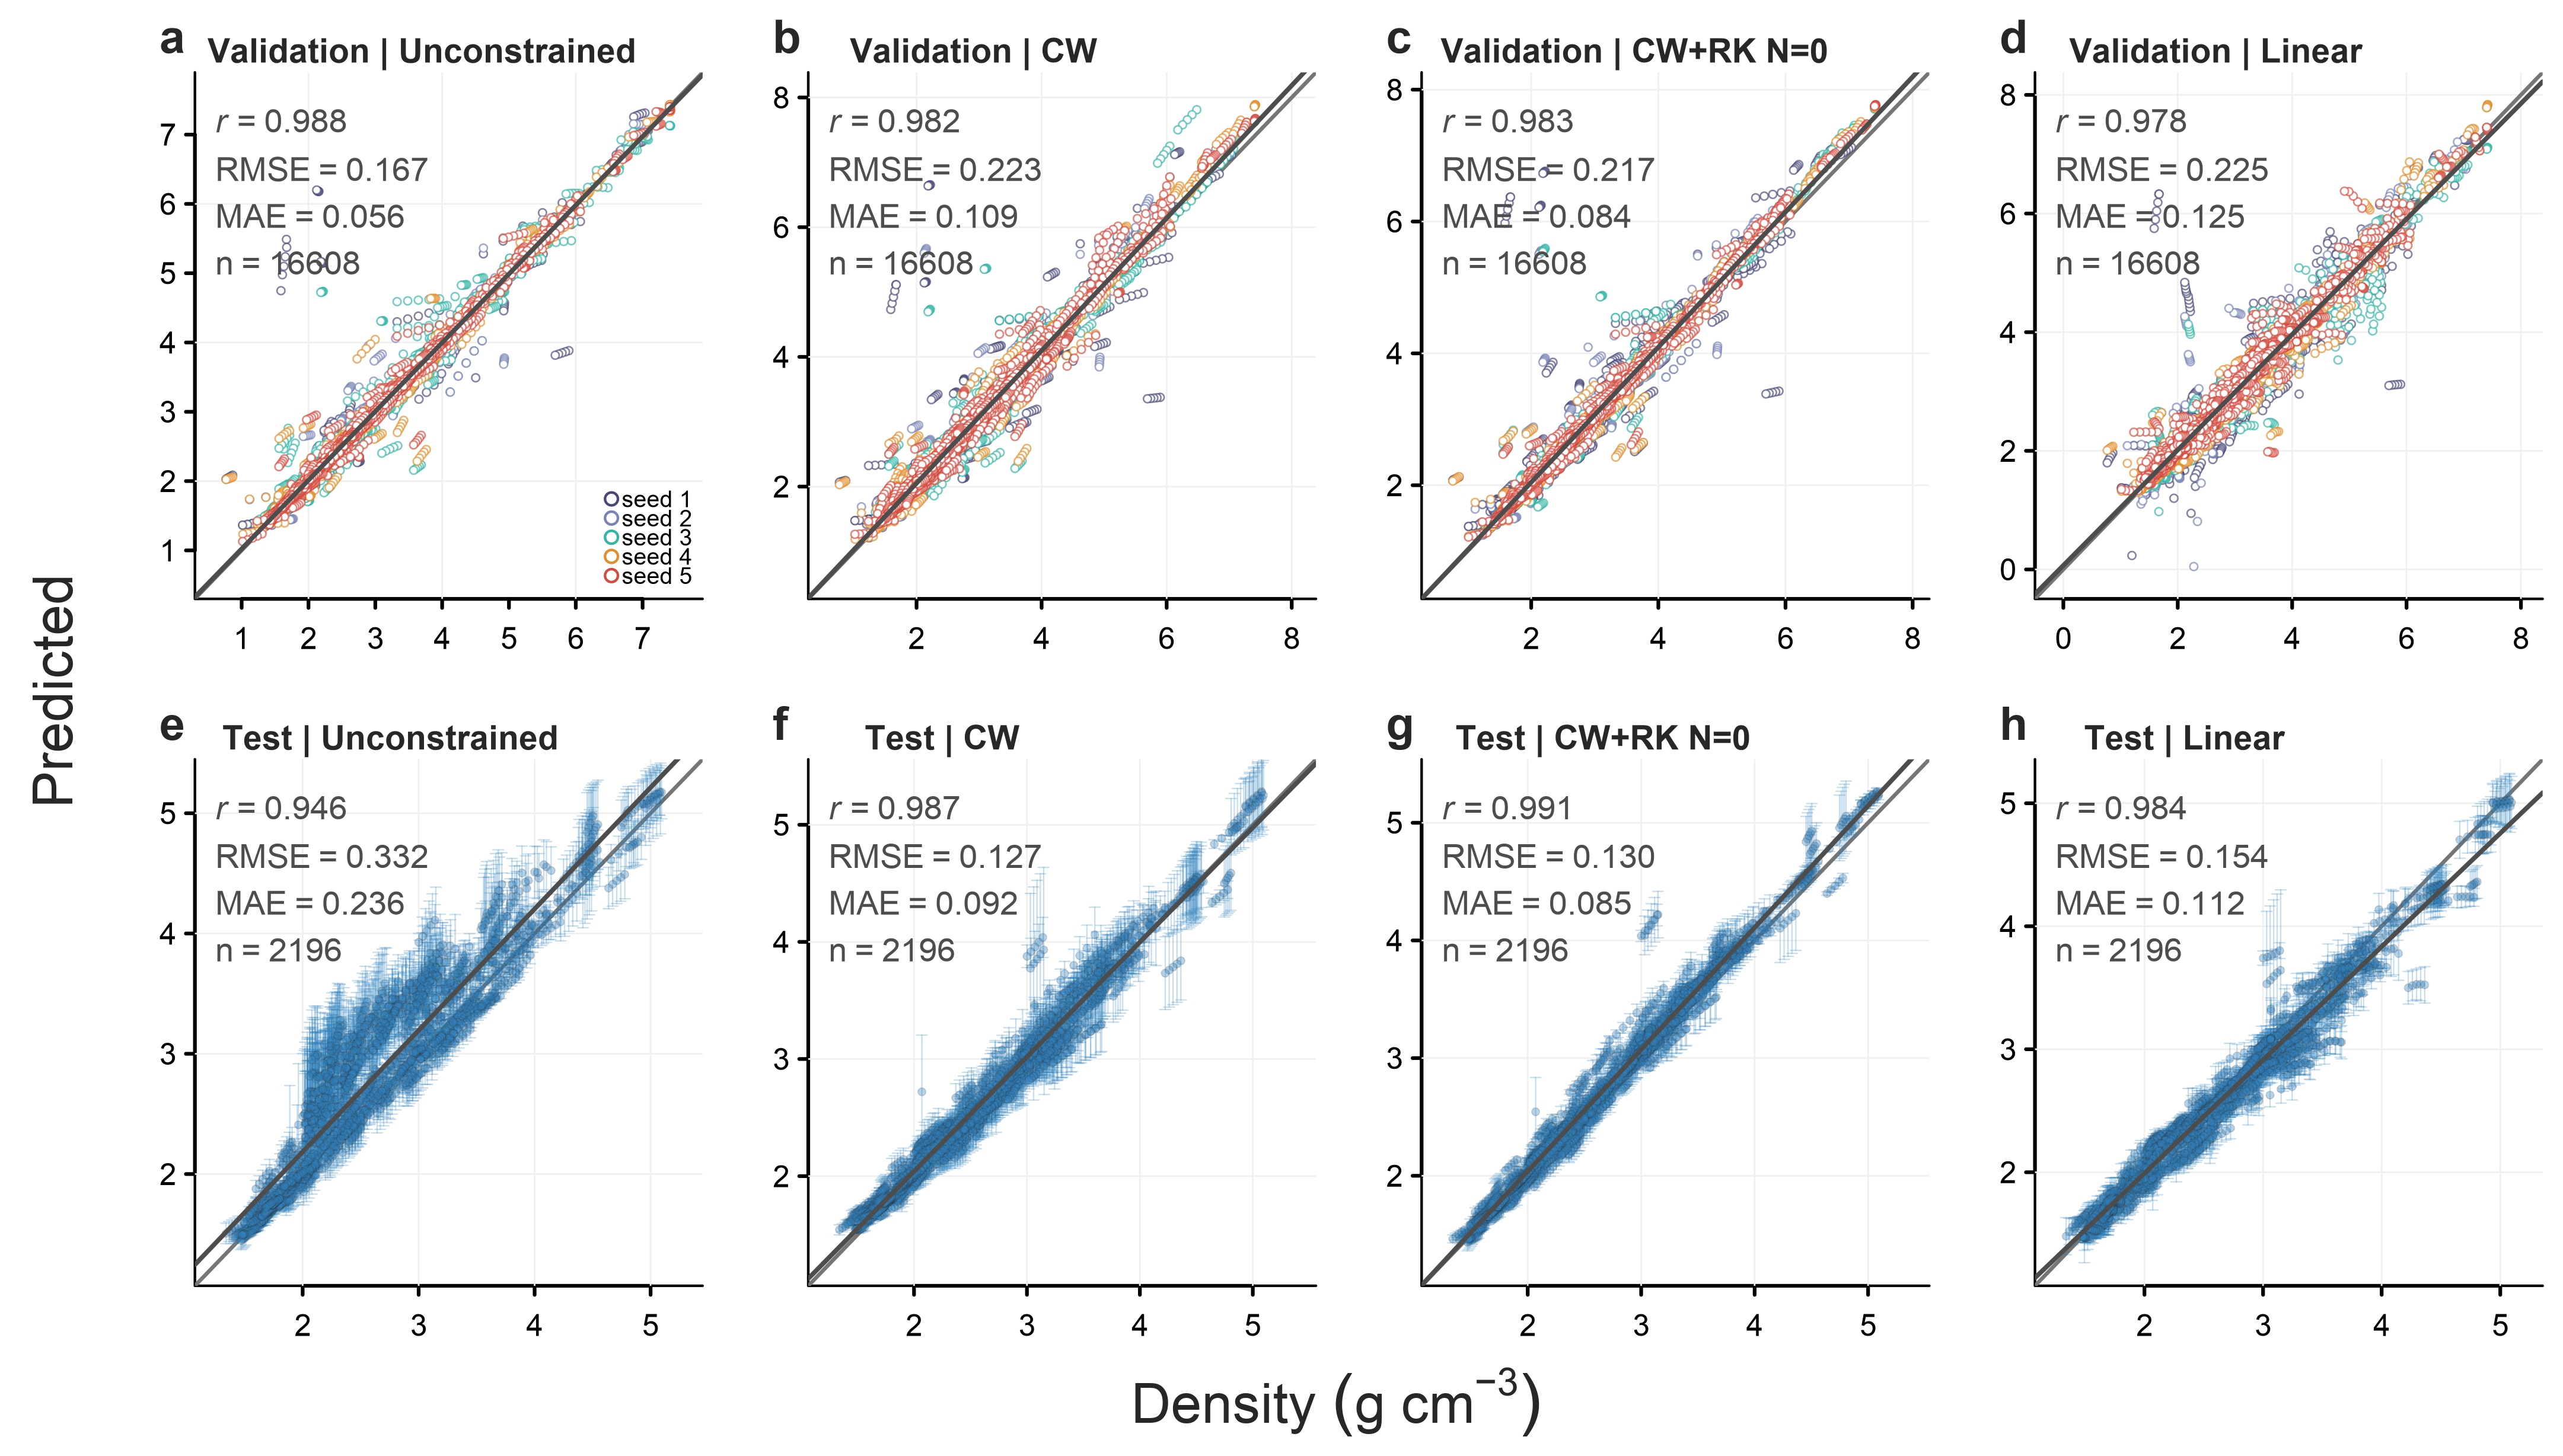
\includegraphics[width=\linewidth]{figures/density_correlation_grid.png}
\caption{密度任务中不同模型变体的预测值与参考值相关性。子图 a--f 为验证集结果，依次对应 unconstrained model、CW、CW+RK \(N=0\)、CW+RK \(N=2\)、CW+RK \(N=4\) 和 linear 模型；子图 g--l 为相同模型顺序下的三元及以上测试集结果。}
\label{fig:density-correlation-grid}
\end{figure}
\FloatBarrier

\subsection{表面张力}\label{ux8868ux9762ux5f20ux529b}

表面张力任务中，linear 模型在一元/二元验证集上表现最稳定，取得最低 Val RMSE 和 MAE 以及最高 Val Pearson \(r\)。这表明线性温度约束能够较好描述低阶体系中的主要表面张力变化趋势，而 RK 修正在该性质中未显示稳定优势。在三元及以上测试集中，不同评价指标给出的最优模型略有差异；对应的预测--参考值相关性见图~\ref{fig:surface-tension-correlation-grid}。Unconstrained model 取得最低 Test RMSE（\(8.75 \pm 1.80\)），而 linear 模型取得最低 Test MAE（\(5.66 \pm 0.88\)）和最高 Test Pearson \(r\)（\(0.98 \pm 0.00\)）。因此，若以整体误差幅度中的 RMSE 为标准，unconstrained model 表现最好；若关注平均误差和趋势相关性，linear 模型更稳定。CW 和 CW+RK 变体在表面张力任务中未形成一致优势，测试性能也未随 RK 阶数提高而系统改善。这说明，对当前表面张力外推任务而言，增加 RK 组成多项式容量并不能稳定提升三元及以上混合物预测性能。

Supporting Information 中的 Figure S3 给出不同随机种子下的 RMSE 和 MAE 分布，Figure S4 按测试体系展示预测--参考值相关性；Table S14 汇总 ternary 测试体系的子体系覆盖情况。体系级误差主要与低阶子体系覆盖不足有关，例如 BeF\(_2\)--LiF--ThF\(_4\) 缺少纯 BeF\(_2\) 和 BeF\(_2\)--ThF\(_4\) 覆盖，模型在该体系中表现出系统性高估。

\begin{figure}[!htbp]
\centering
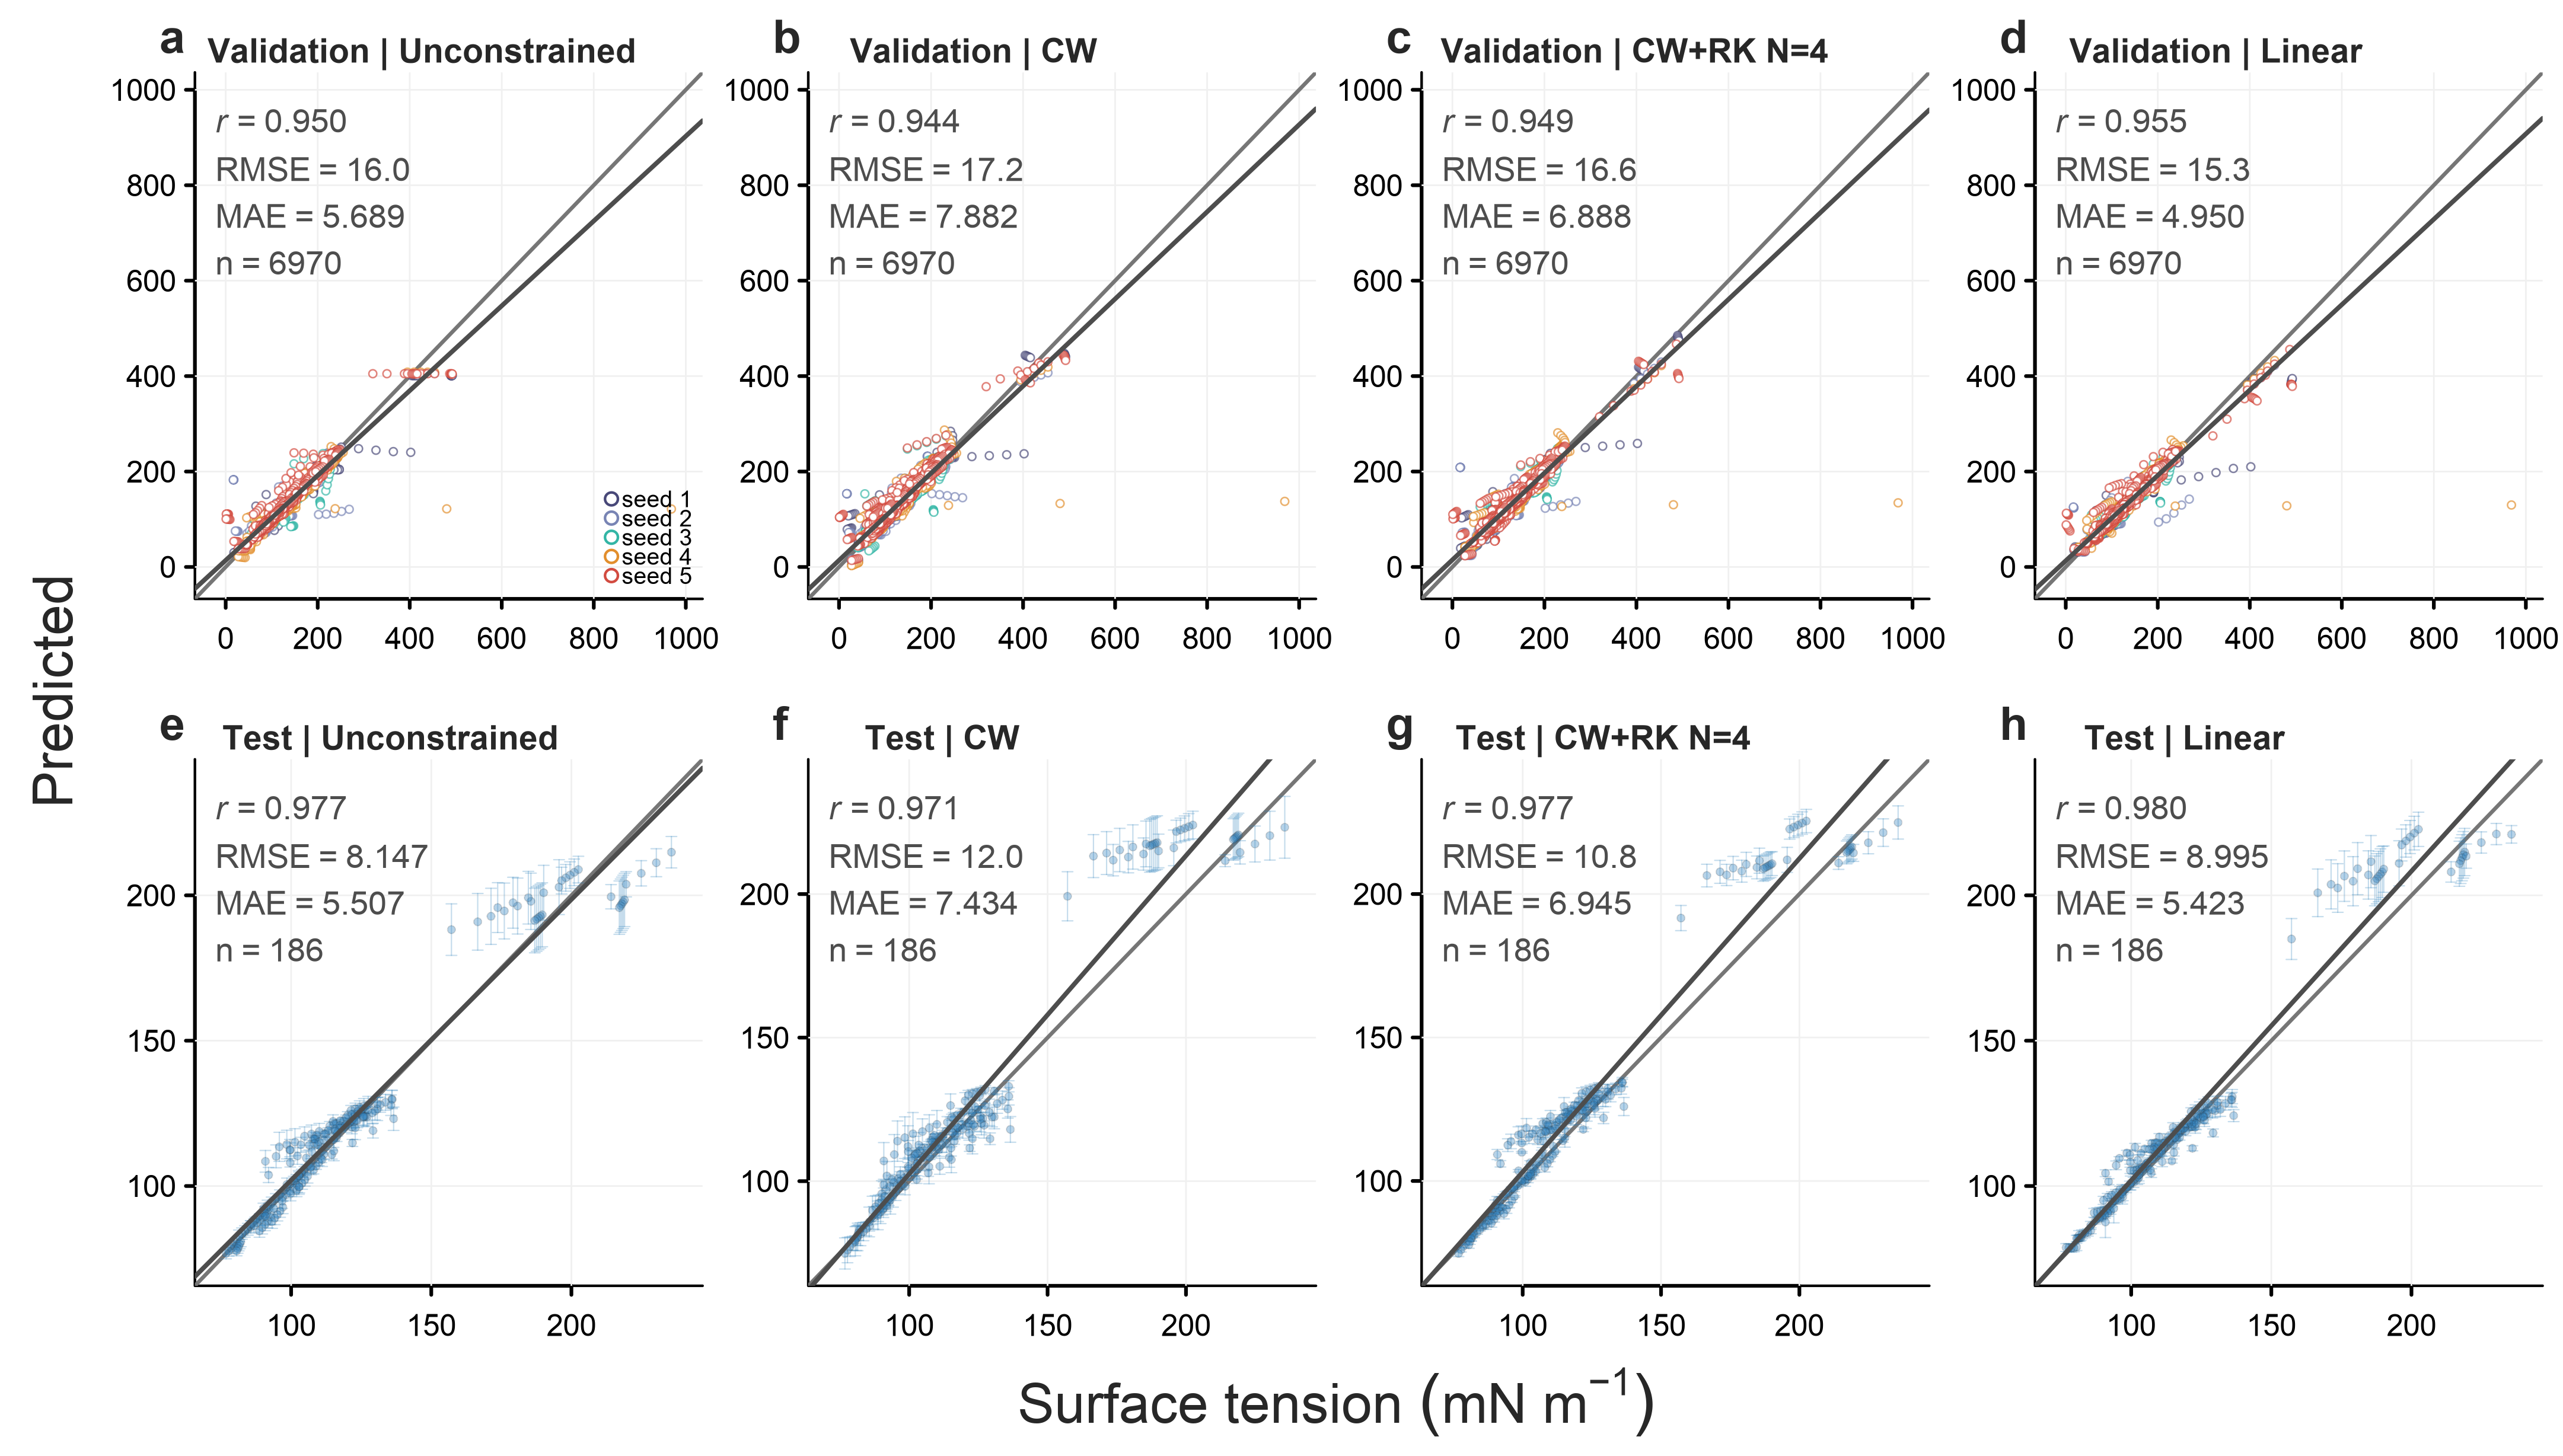
\includegraphics[width=\linewidth]{figures/surface_tension_correlation_grid.png}
\caption{表面张力任务中不同模型变体的预测值与参考值相关性。子图 a--f 为验证集结果，依次对应 unconstrained model、CW、CW+RK \(N=0\)、CW+RK \(N=2\)、CW+RK \(N=4\) 和 linear 模型；子图 g--l 为相同模型顺序下的三元及以上测试集结果。}
\label{fig:surface-tension-correlation-grid}
\end{figure}
\FloatBarrier

\subsection{粘度}\label{ux7c98ux5ea6}

粘度任务中，验证集和三元及以上测试集同样给出不同的模型排序。在一元/二元验证集上，unconstrained model 取得最低 Val RMSE 和 MAE；但在三元及以上测试集中，Arrhenius temperature-constrained model 表现最好，对应的预测--参考值相关性见图~\ref{fig:viscosity-correlation-grid}。Arrhenius 模型的 Test RMSE、Test MAE 和 Test Pearson \(r\) 分别为 \(0.33 \pm 0.04\)、\(0.25 \pm 0.03\) 和 \(0.94 \pm 0.02\)，均优于 unconstrained model、CW 模型和 CW+RK 变体。这表明，对数空间中的 Arrhenius 型温度约束比单纯增加组成混合项更有利于粘度的混合阶数外推。CW+RK 变体未表现出稳定的阶数收益。尽管 CW+RK \(N=4\) 的测试误差低于 \(N=0\) 和 \(N=2\)，其整体表现仍弱于 Arrhenius 模型。因此，对于当前粘度任务，主要外推增益来自温度激活形式约束，而不是更高阶 RK 组成多项式。

Supporting Information 中的 Figure S5 给出不同随机种子下的 RMSE 和 MAE 分布，Figure S6 按测试体系展示预测--参考值相关性；Table S15 和 Table S16 分别汇总 ternary 和 quaternary 测试体系的子体系覆盖情况。体系级误差主要集中在低温高粘度区域和高价组分覆盖不足的体系中，例如 KCl--MgCl\(_2\)--NaCl 在最高对数粘度区域被明显低估，而 LiF--NaF--ZrF\(_4\) 等体系还受到 ZrF\(_4\) 相关覆盖不足的限制。

\begin{figure}[!htbp]
\centering
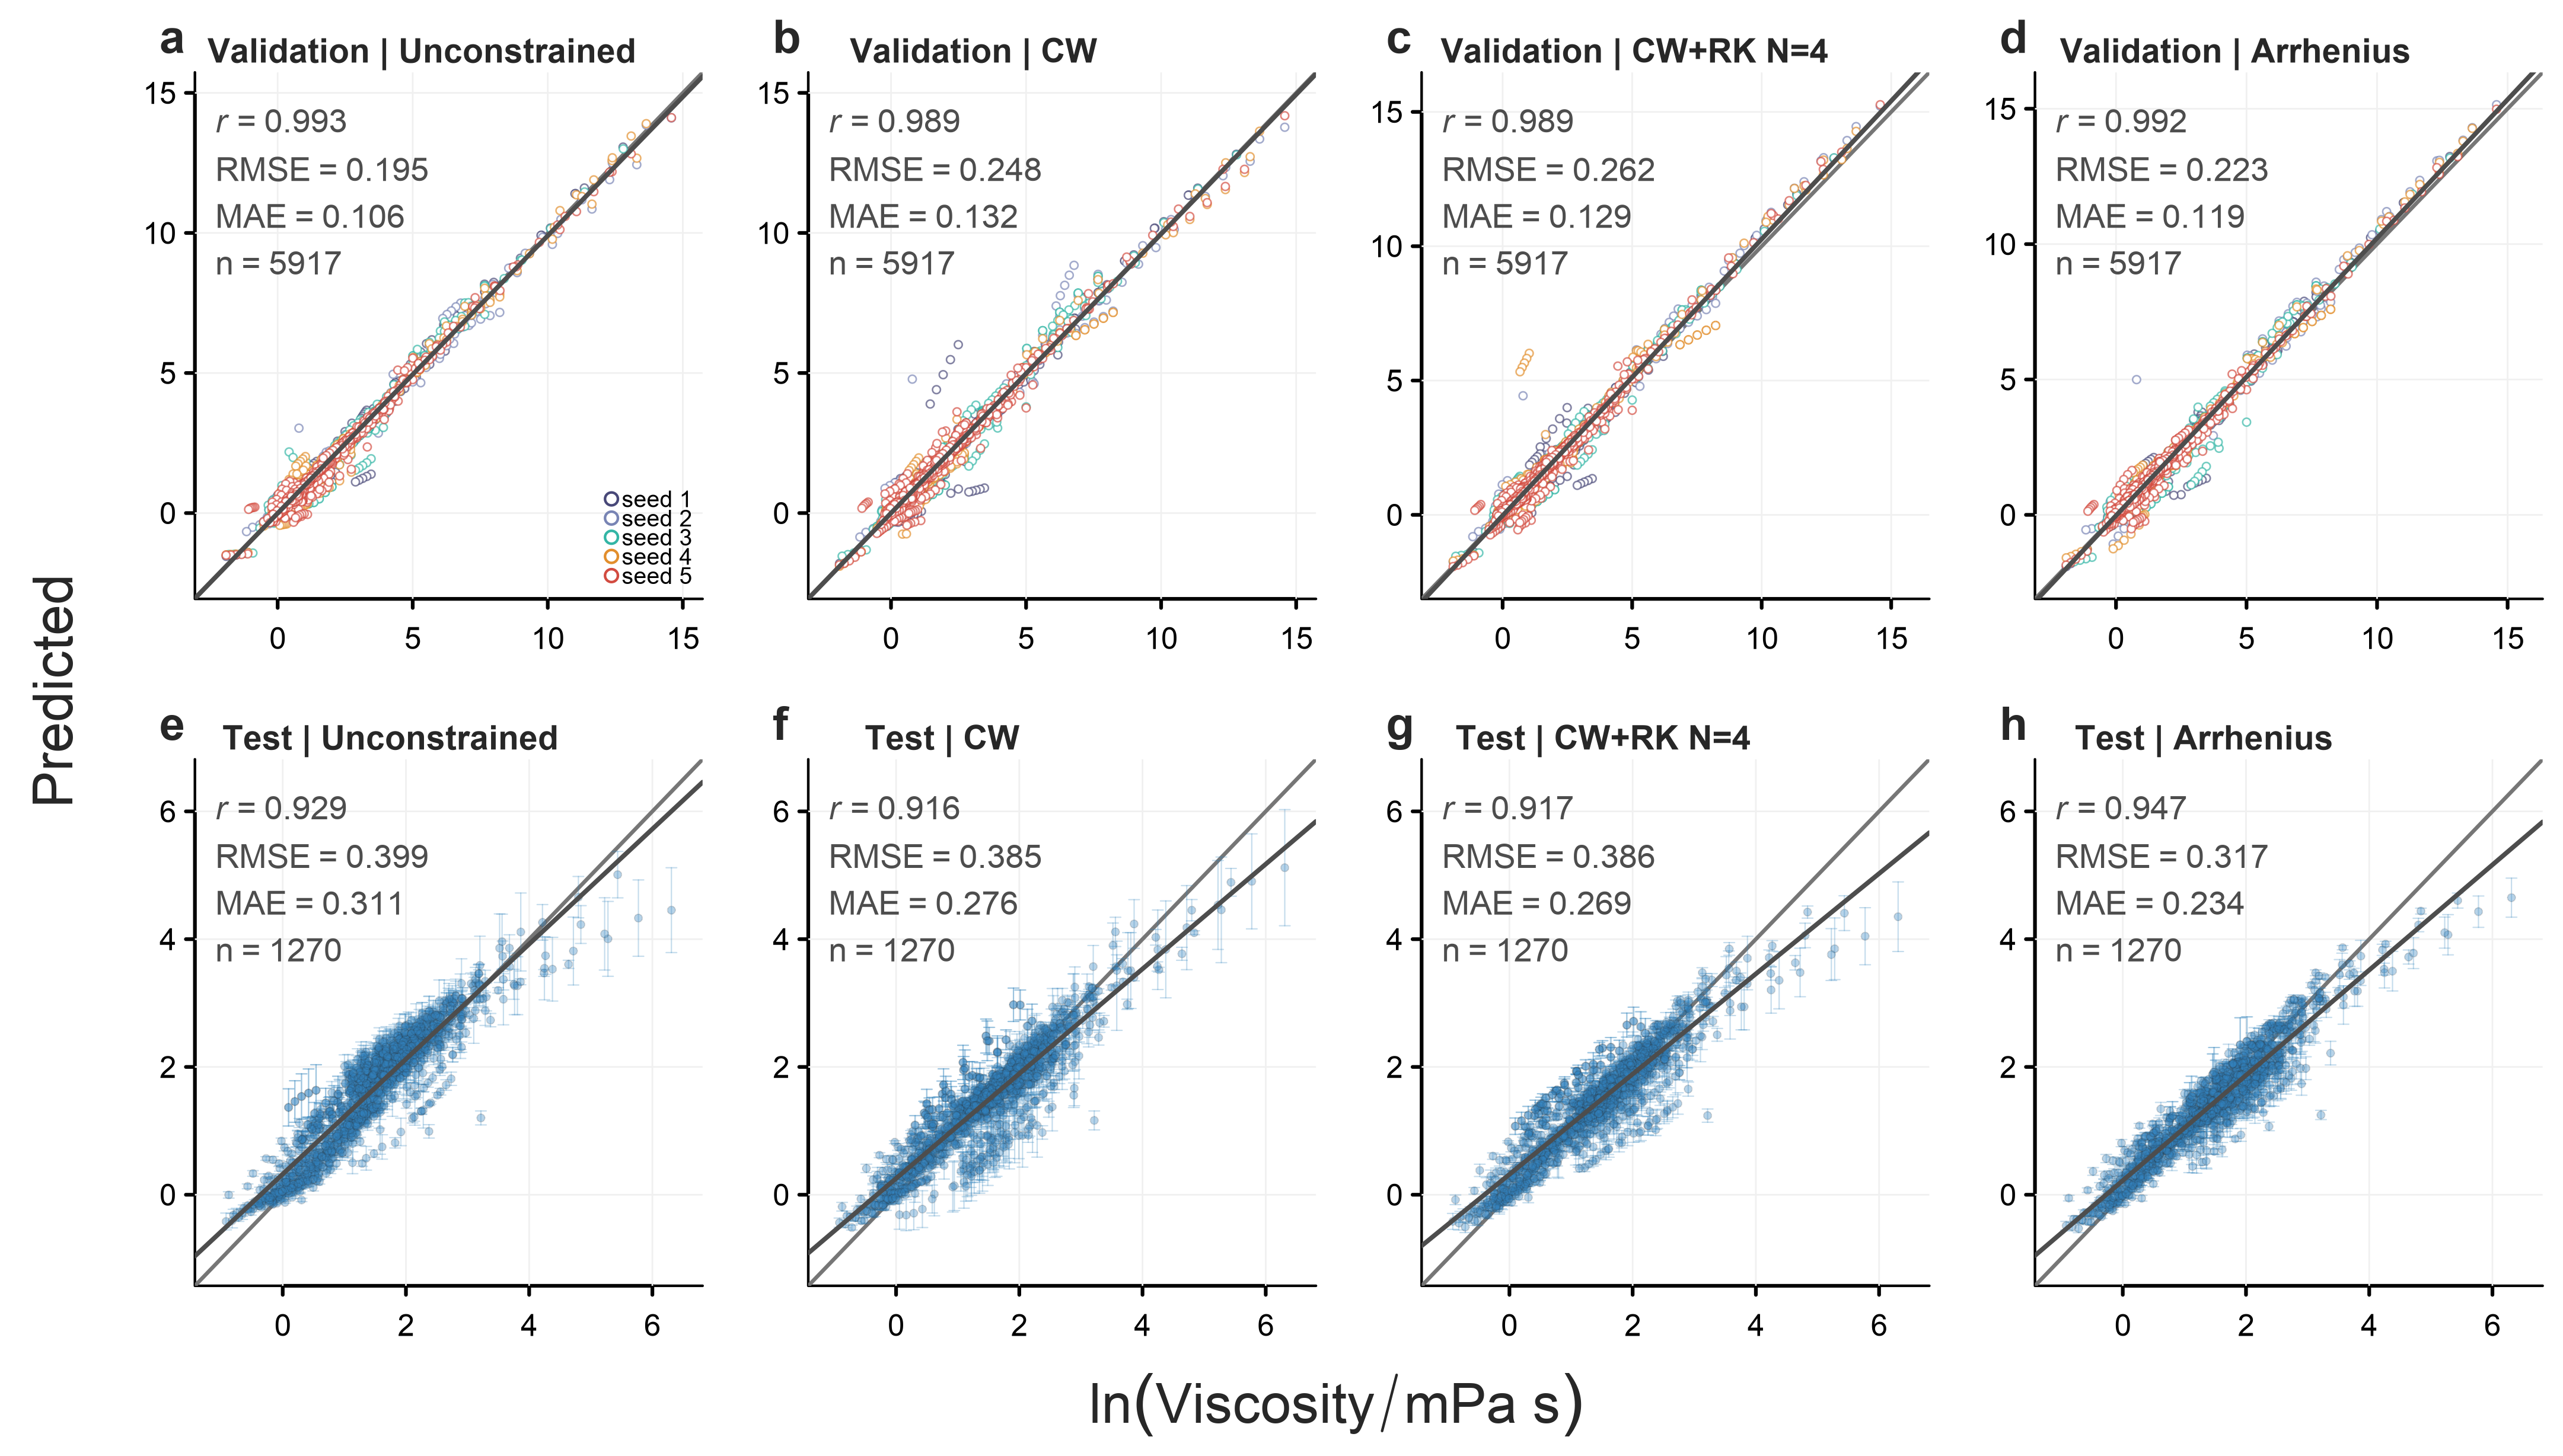
\includegraphics[width=\linewidth]{figures/viscosity_correlation_grid.png}
\caption{粘度任务中不同模型变体的预测值与参考值相关性。子图 a--f 为验证集结果，依次对应 unconstrained model、CW、CW+RK \(N=0\)、CW+RK \(N=2\)、CW+RK \(N=4\) 和 Arrhenius 模型；子图 g--l 为相同模型顺序下的三元及以上测试集结果。}
\label{fig:viscosity-correlation-grid}
\end{figure}
\FloatBarrier

\subsection{电导率}\label{ux7535ux5bfcux7387}

电导率任务中，unconstrained model 在一元/二元验证集上表现最好，取得最低 Val RMSE 和 MAE 以及最高 Val Pearson \(r\)。在三元及以上测试集中，unconstrained model 和 Arrhenius temperature-constrained model 表现接近；对应的预测--参考值相关性见图~\ref{fig:electrical-conductivity-correlation-grid}。Unconstrained model 取得最低 Test RMSE（\(0.38 \pm 0.07\)）和最高 Test Pearson \(r\)（\(0.95 \pm 0.02\)），Arrhenius 模型则取得最低 Test MAE（\(0.25 \pm 0.03\)）。因此，当前电导率任务中的最优模型具有指标依赖性：若以 RMSE 和相关性为标准，unconstrained model 表现最好；若以 MAE 为标准，Arrhenius 模型更优。CW 和 CW+RK 变体未显示稳定优势，且高阶 RK 修正反而导致性能下降。尤其 CW+RK \(N=4\) 的测试误差增大、相关性降低，表明增加 RK 组成多项式容量不能有效改善电导率的混合阶数外推。考虑到电导率测试体系数量相对有限，当前结果更适合解释为：共享组分编码器和集合表示已经具有较强竞争力，而 Arrhenius 约束在平均误差上提供了互补收益；二者不能简单判定为一方整体优于另一方。

Supporting Information 中的 Figure S7 给出不同随机种子下的 RMSE 和 MAE 分布，Figure S8 按测试体系展示预测--参考值相关性；Table S17 汇总 ternary 测试体系的子体系覆盖情况。体系级误差主要来自低阶覆盖缺口导致的低电导率区域外推，例如 CaCrO\(_4\)--KCl--LiCl 缺少纯 CaCrO\(_4\) 和 CaCrO\(_4\)--KCl 覆盖，模型对低电导率样本出现明显高估。

\begin{figure}[!htbp]
\centering
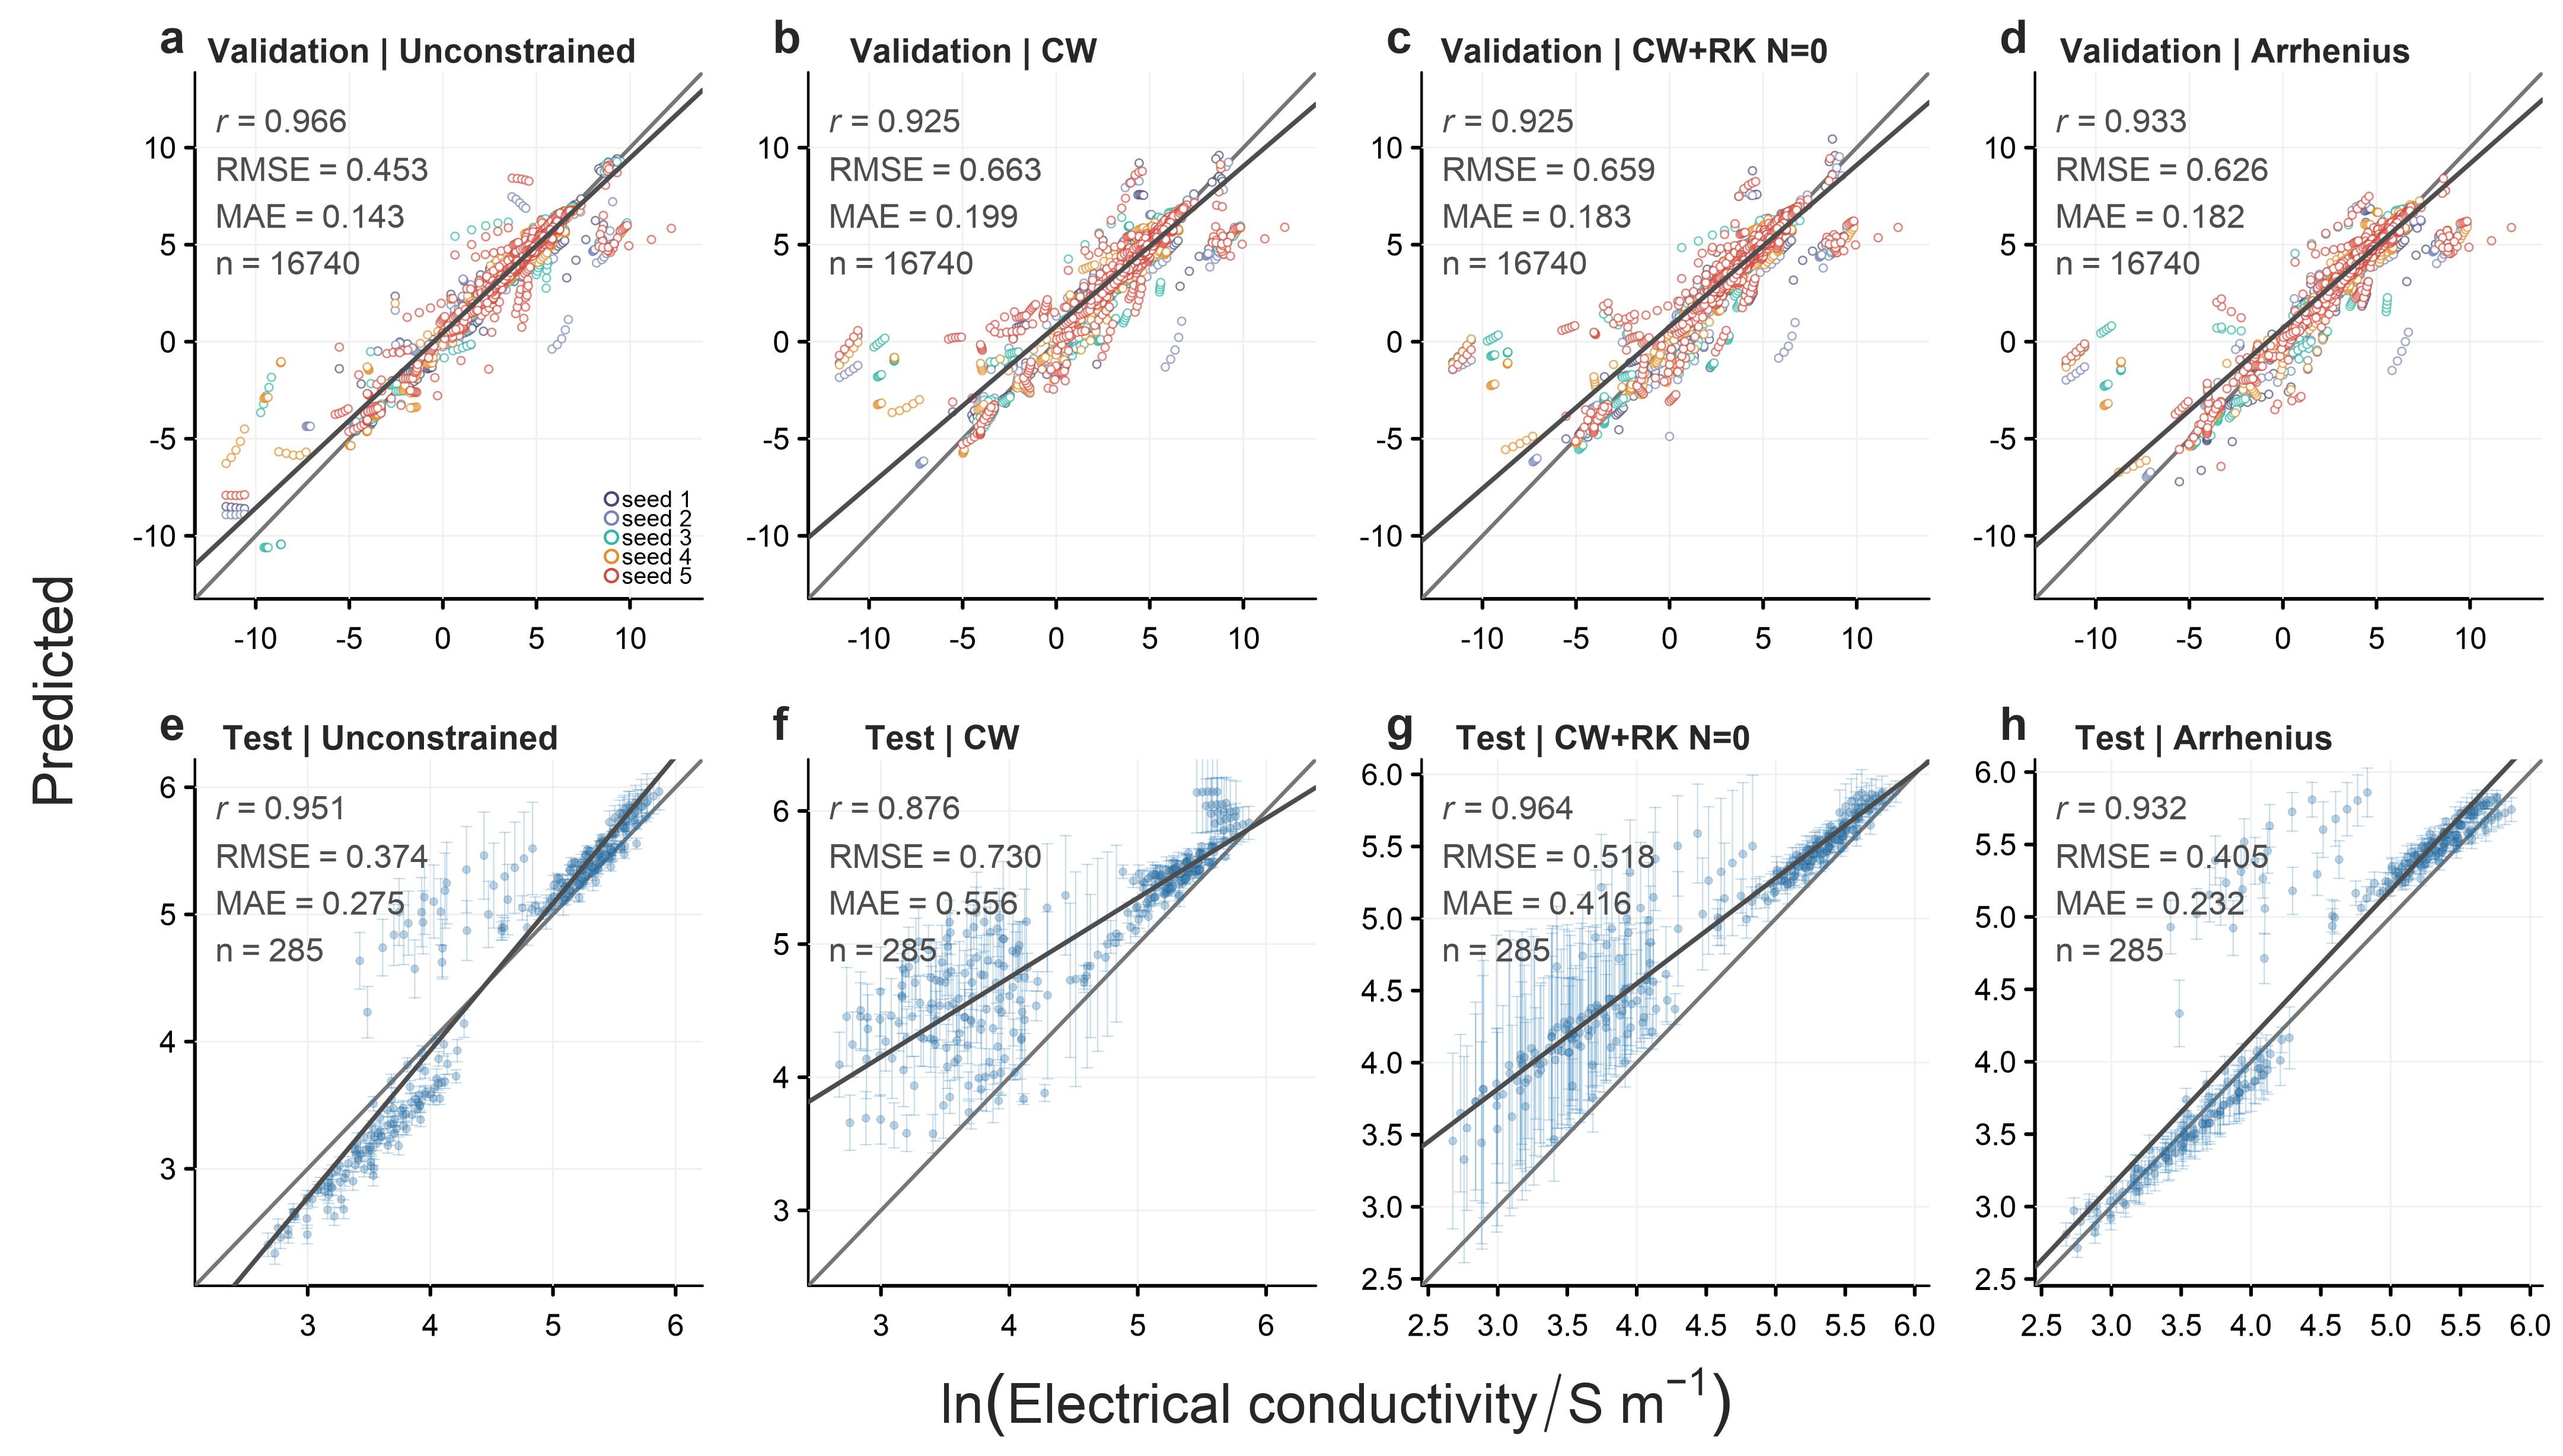
\includegraphics[width=\linewidth]{figures/electrical_conductivity_correlation_grid.png}
\caption{电导率任务中不同模型变体的预测值与参考值相关性。子图 a--f 为验证集结果，依次对应 unconstrained model、CW、CW+RK \(N=0\)、CW+RK \(N=2\)、CW+RK \(N=4\) 和 Arrhenius 模型；子图 g--l 为相同模型顺序下的三元及以上测试集结果。}
\label{fig:electrical-conductivity-correlation-grid}
\end{figure}
\FloatBarrier

\section{讨论}\label{ux8ba8ux8bba}

第三章结果表明，物理启发的归纳偏置并不对所有熔盐物性产生一致收益。其有效性主要取决于约束形式是否与目标物性的主导机制相匹配，而不是约束是否更显式、模型是否更复杂。因此，本文结果更应被理解为不同归纳偏置适用边界的比较，而不是单一模型结构优劣的排序。在本文采用的混合阶数外推设定下，结果主要反映低阶到高阶混合物迁移中的可组合性，而不是对全新离子或全新盐族的外推能力。

\subsection{密度：体相非理想混合与低阶 RK 修正}\label{ux5bc6ux5ea6ux4f53ux76f8ux975eux7406ux60f3ux6df7ux5408ux4e0e-rk-ux4feeux6b63}

密度与摩尔体积、离子 packing 和体相混合结构密切相关。熔盐混合物密度偏离简单加和时，通常与离子尺寸差异、局域配位变化、盐对之间的 packing 效应以及过量体积有关。RK 展开本身适合描述二元混合物中的低阶过量性质和非理想混合效应 \cite{redlich1948algebraic,birri2022redlich,birri2024viscosity,prausnitz1999molecular}，因此在密度任务中，RK 项可以被理解为组成加权项上的成对非理想修正。类似思想也已用于熔盐之外的液态离子体系性质建模，如电解液混合物 \cite{zhu2024diffmix}。

需要强调的是，本文的 RK 修正直接作用于密度目标空间，而不是显式摩尔体积空间。因此，它不是严格热力学意义上的过量体积模型，而是由组分表示条件化的低阶非理想修正。在当前数据覆盖下，低阶 RK 项已经能够捕捉主要的成对混合偏差；进一步提高 RK 阶数虽然增加了组成空间表达能力，但也可能在高阶测试体系有限时引入额外方差。这解释了为什么低阶 RK 修正对密度更有效，而更高阶 RK 多项式没有形成稳定收益。

\subsection{表面张力：界面性质与线性温度趋势}\label{ux8868ux9762ux5f20ux529bux754cux9762ux6027ux8d28ux4e0eux7ebfux6027ux6e29ux5ea6ux8d8bux52bf}

表面张力不同于密度，它是界面性质，不完全由体相成对混合项决定。除整体组成外，表面张力还受到界面层组成重排、表面富集、长程库仑作用以及低表面张力组分优先占据界面的影响。Goodisman 对熔盐混合物表面张力的分析指出，混合熔盐表面张力常低于按摩尔分数加权得到的纯盐表面张力平均值，其中低表面张力组分的表面富集和长程相互作用均可能产生贡献 \cite{goodisman1980surface}。

因此，linear 模型在表面张力任务中的优势不应被解释为表面张力在物理上完全线性，而应理解为：在当前数据范围内，主要可学习变化更接近稳定的一阶组成--温度趋势。相比之下，RK 多项式主要表达体相组成非理想性，不能直接描述界面富集、界面层重排和表面选择性吸附等过程。当额外的组成非线性自由度与真实界面机制不匹配时，模型容量增加并不必然带来更好的外推稳定性。

\subsection{粘度与电导率：输运性质与温度激活}\label{ux7c98ux5ea6ux4e0eux7535ux5bfcux7387ux8f93ux8fd0ux6027ux8d28ux4e0eux6e29ux5ea6ux6fc0ux6d3b}

粘度和电导率都属于输运性质，其主导因素不同于密度和表面张力。二者并非简单的平衡混合量，而是与离子迁移、局域结构松弛、相互作用网络重排以及温度驱动的活化过程相关。粘度反映熔盐体系发生结构重排和流动时的阻力，通常与流动活化能有关，其温度依赖可由 Arrhenius 或类 Arrhenius 形式近似描述 \cite{janz1988molten,zhao2023viscosity}。因此，对于粘度，显式引入 Arrhenius 型温度依赖比增加 RK 组成多项式更直接地对应其主导物理过程。

电导率的情况更复杂。电导率不仅取决于温度激活，还受到载流离子迁移率、离子缔合、局域结构和相关运动的共同影响。Walz 和 van der Spoel 的模拟研究也表明，熔盐电导率的微观来源需要同时考虑离子电迁移率、局域结构和动力学过程，高电导率并不必然等同于某一离子的高迁移率 \cite{walz2021microscopic}。这解释了为什么 Arrhenius 约束在电导率中具有竞争力，但并不能完全替代更灵活的神经集合表示。换言之，电导率同时包含温度激活趋势和复杂组成依赖，单一温度函数约束不足以覆盖全部变化来源。

\section{总结}\label{ux603bux7ed3}

本文构建并系统比较了一套物理启发的组分编码神经网络模型，用于评估多元熔盐物性在混合阶数外推场景下的预测能力。该框架将盐的化学式、阳离子、阴离子及其化学计量关系转化为结构化序列表示，并在统一的数据表示与评估协议下，对比 CW/CW+RK 组成混合模型和 linear/Arrhenius 温度约束模型。为考察模型从低阶混合物向高阶混合物迁移的能力，本文采用“一元/二元体系训练、三元及以上体系测试”的外推设定，评估模型能否将在一元和二元体系中学习到的组成--温度--物性关系推广至更高阶混合物。

实验结果表明，不同熔盐物性的最优归纳偏置并不相同。密度更受益于低阶 RK 修正，说明成对非理想混合项能够改善体相混合性质的高阶外推；表面张力中，linear 模型在 MAE 和相关性上更稳定，而 unconstrained model 在 RMSE 上表现最好；粘度中，Arrhenius 模型在测试集各项指标上均表现最优；电导率中，unconstrained model 和 Arrhenius 模型表现接近，且优势随评价指标而变化。这些结果共同说明，高阶熔盐物性外推不宜依赖统一的物理约束形式，而应根据目标性质的主导机制选择归纳偏置。

总体来看，低阶 RK 修正更适合体相非理想混合相关性质，linear 温度约束可稳定刻画表面张力的主要趋势，Arrhenius 约束对温度激活主导的粘度更有效，而电导率需要在温度依赖先验和灵活数据驱动表示之间权衡。该结论为有限低阶数据条件下的高阶熔盐物性预测提供了性质导向的模型选择基线。同时，本文结论仍受经验关联式数据来源、数据覆盖范围和低阶子体系覆盖情况限制。后续工作可结合独立实验数据进一步评估模型在更广泛化学空间中的可靠性。

\begin{suppinfo}
The Supporting Information includes system--property distribution tables for the Janz and MSTDB-TP(v4) datasets; a table of manually curated Janz records; a JSON example of the structured salt-component sequence together with cation and anion token lists; supplemental model-performance figures comparing RMSE/MAE across model variants and RK orders and showing test-system prediction--reference correlations; and subsystem-coverage tables for the density, surface tension, viscosity, and electrical-conductivity test systems, with quaternary coverage reported where such test systems are present.
\end{suppinfo}

\renewcommand{\refname}{参考文献}
\bibliography{references}

\end{document}
